\documentclass[11pt]{article}

\usepackage[margin=1in]{geometry}
\usepackage{amsmath}
\usepackage{array}
\usepackage{graphicx}
\usepackage{float}
\usepackage[colorlinks=true,linkcolor=blue,urlcolor=blue,citecolor=blue]{hyperref}

\newcommand{\E}{\operatorname{E}}
\newcommand{\Var}{\operatorname{Var}}
\newcommand{\RMSE}{\operatorname{RMSE}}
\newcommand{\CV}{\operatorname{CV}}
\newcommand{\Wcal}{\mathcal{W}}

\title{Comparison of Geometric and Energy-Based Error Scaling\\
for Recursive Intrinsic Multiscale Filtering}
\author{}
\date{}

\begin{document}
\maketitle

\section{Task}

The notebook \texttt{gd\_imf\_real\_vs\_calculated.ipynb} scales every
stage-$k$ error by the geometric factor $a^{k/2}$, where $a=\sqrt{2}$ is the
bandwidth reduction factor. The companion notebook
\path{gd_imf_real_vs_calculated_energy_scaled.ipynb}, stored under
\path{output/jupyter-notebook/}, uses a stage-specific error scale derived from
the energy of the complete recursive filter. For the nonlinear robust
decomposition, the corresponding scale is estimated by a parametric bootstrap.

The methods answer different questions:

\begin{itemize}
    \item \emph{Geometric scaling}: does the error follow the theoretical
    bandwidth order $(nh_k)^{-1/2}$?
    \item \emph{Energy scaling}: is the error consistent with the variance of
    the complete stage-specific operator, including all previous residual
    subtractions?
\end{itemize}

The comparison should therefore consider calibration, assumptions, and
computational cost in addition to visual flatness.

\section{Common Error Quantities}

Let $W_k$ denote the local linear smoother at IMF stage $k$, and define the
residual operator
\[
A_{k-1}=(I-W_{k-1})\cdots(I-W_1),
\qquad A_0=I.
\]
The complete recursive component operator is
\[
\Wcal_k=W_kA_{k-1}.
\]
For an observation $Y=X+\varepsilon$, the linear recursive component error is
\[
e_k=\widetilde S^{(k)}-S^{(k)}=\Wcal_k\varepsilon.
\]
The first component is low-pass because $A_0=I$. Later recursive components are
band-pass because $A_{k-1}$ removes the low-frequency content extracted at the
previous stages.

The main scalar diagnostics are
\[
\RMSE(e_k)=\left\{\frac{1}{n}\sum_{t=1}^n e_k(t)^2\right\}^{1/2},
\qquad
\lVert e_k\rVert_\infty=\max_t |e_k(t)|.
\]

\section{Method 1: Geometric Bandwidth Scaling}

The bandwidth schedule is approximately
\[
h_k=\frac{h_1}{a^{k-1}},
\qquad a=\sqrt{2}.
\]
The original notebook defines
\[
e_k^{\mathrm{geo}}=\frac{e_k}{a^{k/2}}.
\]
The natural stage-one convention would use $a^{(k-1)/2}$, but the two choices
differ by the same constant $a^{1/2}$ at every stage. The indexing convention
cannot create or remove a stage-one discontinuity.

The variance order $1/(nh)$ is standard in kernel and local-polynomial
regression; see, for example, Fan and Gijbels~\cite{fan-gijbels1996} and
Tsybakov~\cite{tsybakov2009}. The underlying kernel estimator was introduced
independently by Nadaraya~\cite{nadaraya1964} and Watson~\cite{watson1964}.
For a regular design, a normalized kernel average with bandwidth $h$ has the
asymptotic variance
\[
\Var\{\widetilde S_h(t)-S_h(t)\}
\approx
\frac{\sigma^2}{nh}
\frac{\int K(u)^2\,du}{\left\{\int K(u)\,du\right\}^2}.
\]
This expression assumes that the number of observations in a window grows,
$nh\to\infty$, and that the noise values have a common variance and are
uncorrelated. The design-density term that appears in the random-design formula
is constant here and is absorbed into the multiplicative constant.

For a recursive IMF component, the relevant operator is not one kernel average
but $\Wcal_k=W_kA_{k-1}$. Lemma 2.5 of the supplied IMF draft
\cite{spokoiny2026} states the corresponding order
\[
\Var\{e_k(t)\}
\asymp \frac{\sigma^2}{nh_k}.
\]
Here $\asymp$ means that the two sides have the same order up to positive
multiplicative constants; it does not mean equality. Writing the stage-specific
constant explicitly gives
\[
\Var\{e_k(t)\}
\approx \frac{\sigma^2}{nh_k}C_k.
\]
The constant $C_k$ contains the squared energy of the complete recursive filter,
including the previous residual operators. This is the recursive analogue of
the kernel-dependent constant in the Nadaraya--Watson variance formula.
Geometric scaling compensates for $h_k^{-1/2}$ but leaves $\sqrt{C_k}$ in the
scaled error, so it checks the bandwidth rate rather than equality of stage
constants.

For the current recursive filters, $C_1$ is about $0.90$, while the later
constants are about $0.09$. A factor of approximately
\[
\sqrt{0.90/0.09}=\sqrt{10}\approx3.16
\]
can remain after geometric scaling without contradicting the common bandwidth
order.

Geometric scaling is useful when the goal is to check the predicted bandwidth
rate with a simple deterministic normalization. It should not be expected to
make the recursive error curve flat, because it does not remove $C_k$ and hence
does not account for the difference between the first low-pass component and the
later band-pass components. The same rate also does not calibrate a sup error.

\section{Method 2: Stage-Specific Energy Scaling}

\subsection{Exact linear scaling}

Assume that every noise value has mean zero and the same variance $\sigma^2$,
and that different noise values are uncorrelated:
\[
\Var(\varepsilon_t)=\sigma^2,
\qquad
\operatorname{Cov}(\varepsilon_t,\varepsilon_u)=0\quad(t\ne u).
\]
Let $\ell_{k,q}$ be the effective weight placed on the noise value at offset $q$
by the complete recursive stage. In other words,
\[
e_k(t)=\sum_q \ell_{k,q}\varepsilon_{t+q}.
\]
With the notebook's wrap boundary, the same weights are shifted around the time
grid at every $t$. It follows directly that
\[
\Var\{e_k(t)\}
=\sigma^2(\Wcal_k\Wcal_k^\top)_{tt}
=\sigma^2\sum_q\ell_{k,q}^2.
\]
The exact recursive energy scale is
\[
s_{k,\mathrm{rec}}
=\sigma\left(\sum_q\ell_{k,q}^2\right)^{1/2},
\]
and the standardized error is
\[
z_{k,\mathrm{rec}}
=\frac{e_k}{s_{k,\mathrm{rec}}}.
\]
For a periodic regular design, all rows of $\Wcal_k$ have the same norm, so
\[
\E\!\left[\RMSE(z_{k,\mathrm{rec}})^2\right]=1.
\]
This normalization removes both the bandwidth factor and the stage-specific
operator-energy constant.

\subsection{Bootstrap robust scaling}

The robust smoother is nonlinear, so there is no fixed global matrix
$\Wcal_k$. The companion notebook estimates the scale under the same clean
signal, Gaussian noise, signed contamination law, robust loss, window schedule,
and clean-fit reference as the displayed experiment.

For bootstrap replicate $b=1,\ldots,B$, let $e_k^{(b)}(t)$ be the robust
recursive error. The estimated scale is
\[
\widehat s_{k,\mathrm{rec}}
=\left\{
\frac{1}{B}\sum_{b=1}^{B}
\frac{1}{n}\sum_{t=1}^{n}
\left(e_k^{(b)}(t)\right)^2
\right\}^{1/2}.
\]
The displayed error is standardized as
\[
\widehat z_{k,\mathrm{rec}}
=\frac{e_k}{\widehat s_{k,\mathrm{rec}}}.
\]
The current notebook uses $B=32$ deterministic replicates for a quick
reproducible analysis.
For publication-level scale estimates, a larger value such as $B\geq200$ and a
Monte Carlo uncertainty assessment are preferable.

Energy scaling is intended as a calibration rather than only a rate check. In the
linear case it gives an exact unit target for the expected squared standardized
RMSE. In the robust case it is necessarily model-dependent: the result changes
with the signal, contamination law, robust-loss parameter, reference definition,
and bootstrap size. It is therefore more expensive and less universal than the
geometric normalization, and its RMS scale still does not calibrate sup errors.

\section{Relationship Between the Methods}

If
\[
s_k^2
\approx \frac{\sigma^2}{nh_k}C_k,
\]
then, because $h_k\approx h_1a^{-(k-1)}$,
\[
\frac{e_k}{a^{k/2}}
\quad\text{retains a factor proportional to}\quad
\sqrt{C_k},
\]
whereas
\[
\frac{e_k}{s_k}
\]
removes both the bandwidth rate and $C_k$. Thus the methods are complementary:
the first tests theoretical order, while the second tests stage-specific
calibration.

\begin{table}[H]
\centering
\small
\begin{tabular}{@{}>{\raggedright\arraybackslash}p{0.22\linewidth}
>{\raggedright\arraybackslash}p{0.33\linewidth}
>{\raggedright\arraybackslash}p{0.33\linewidth}@{}}
\hline
Criterion & Geometric scaling & Energy scaling \\
\hline
Primary question & Does error follow the bandwidth rate? & Is error calibrated to the complete stage operator? \\
Denominator & $a^{k/2}$ & $\sigma\lVert\ell_k\rVert_2$ or bootstrap estimate \\
Stage-dependent constant & Remains in the result & Included in the denominator \\
Stage 1 & Compared directly with later details & Assigned its own low-pass energy scale \\
Linear computation & Constant time once $k$ is known & Exact FFT/impulse-response calculation \\
Robust computation & No additional computation & Parametric bootstrap or Jacobian/sandwich approximation \\
Expected calibrated RMSE & No unit target & Approximately one \\
Sup-error interpretation & Not calibrated & Still not calibrated by an RMS scale \\
Model dependence & Low & Higher, especially for robust bootstrap \\
\hline
\end{tabular}
\caption{Conceptual comparison of the two error normalizations.}
\end{table}

\section{Empirical Comparison}

Table~\ref{tab:stage-values} gives the recursive RMSE series under both methods.
The columns have different units: geometric values retain the units of the
original signal up to the dimensionless bandwidth factor, while energy-scaled
values are dimensionless.

\begin{figure}[H]
\centering
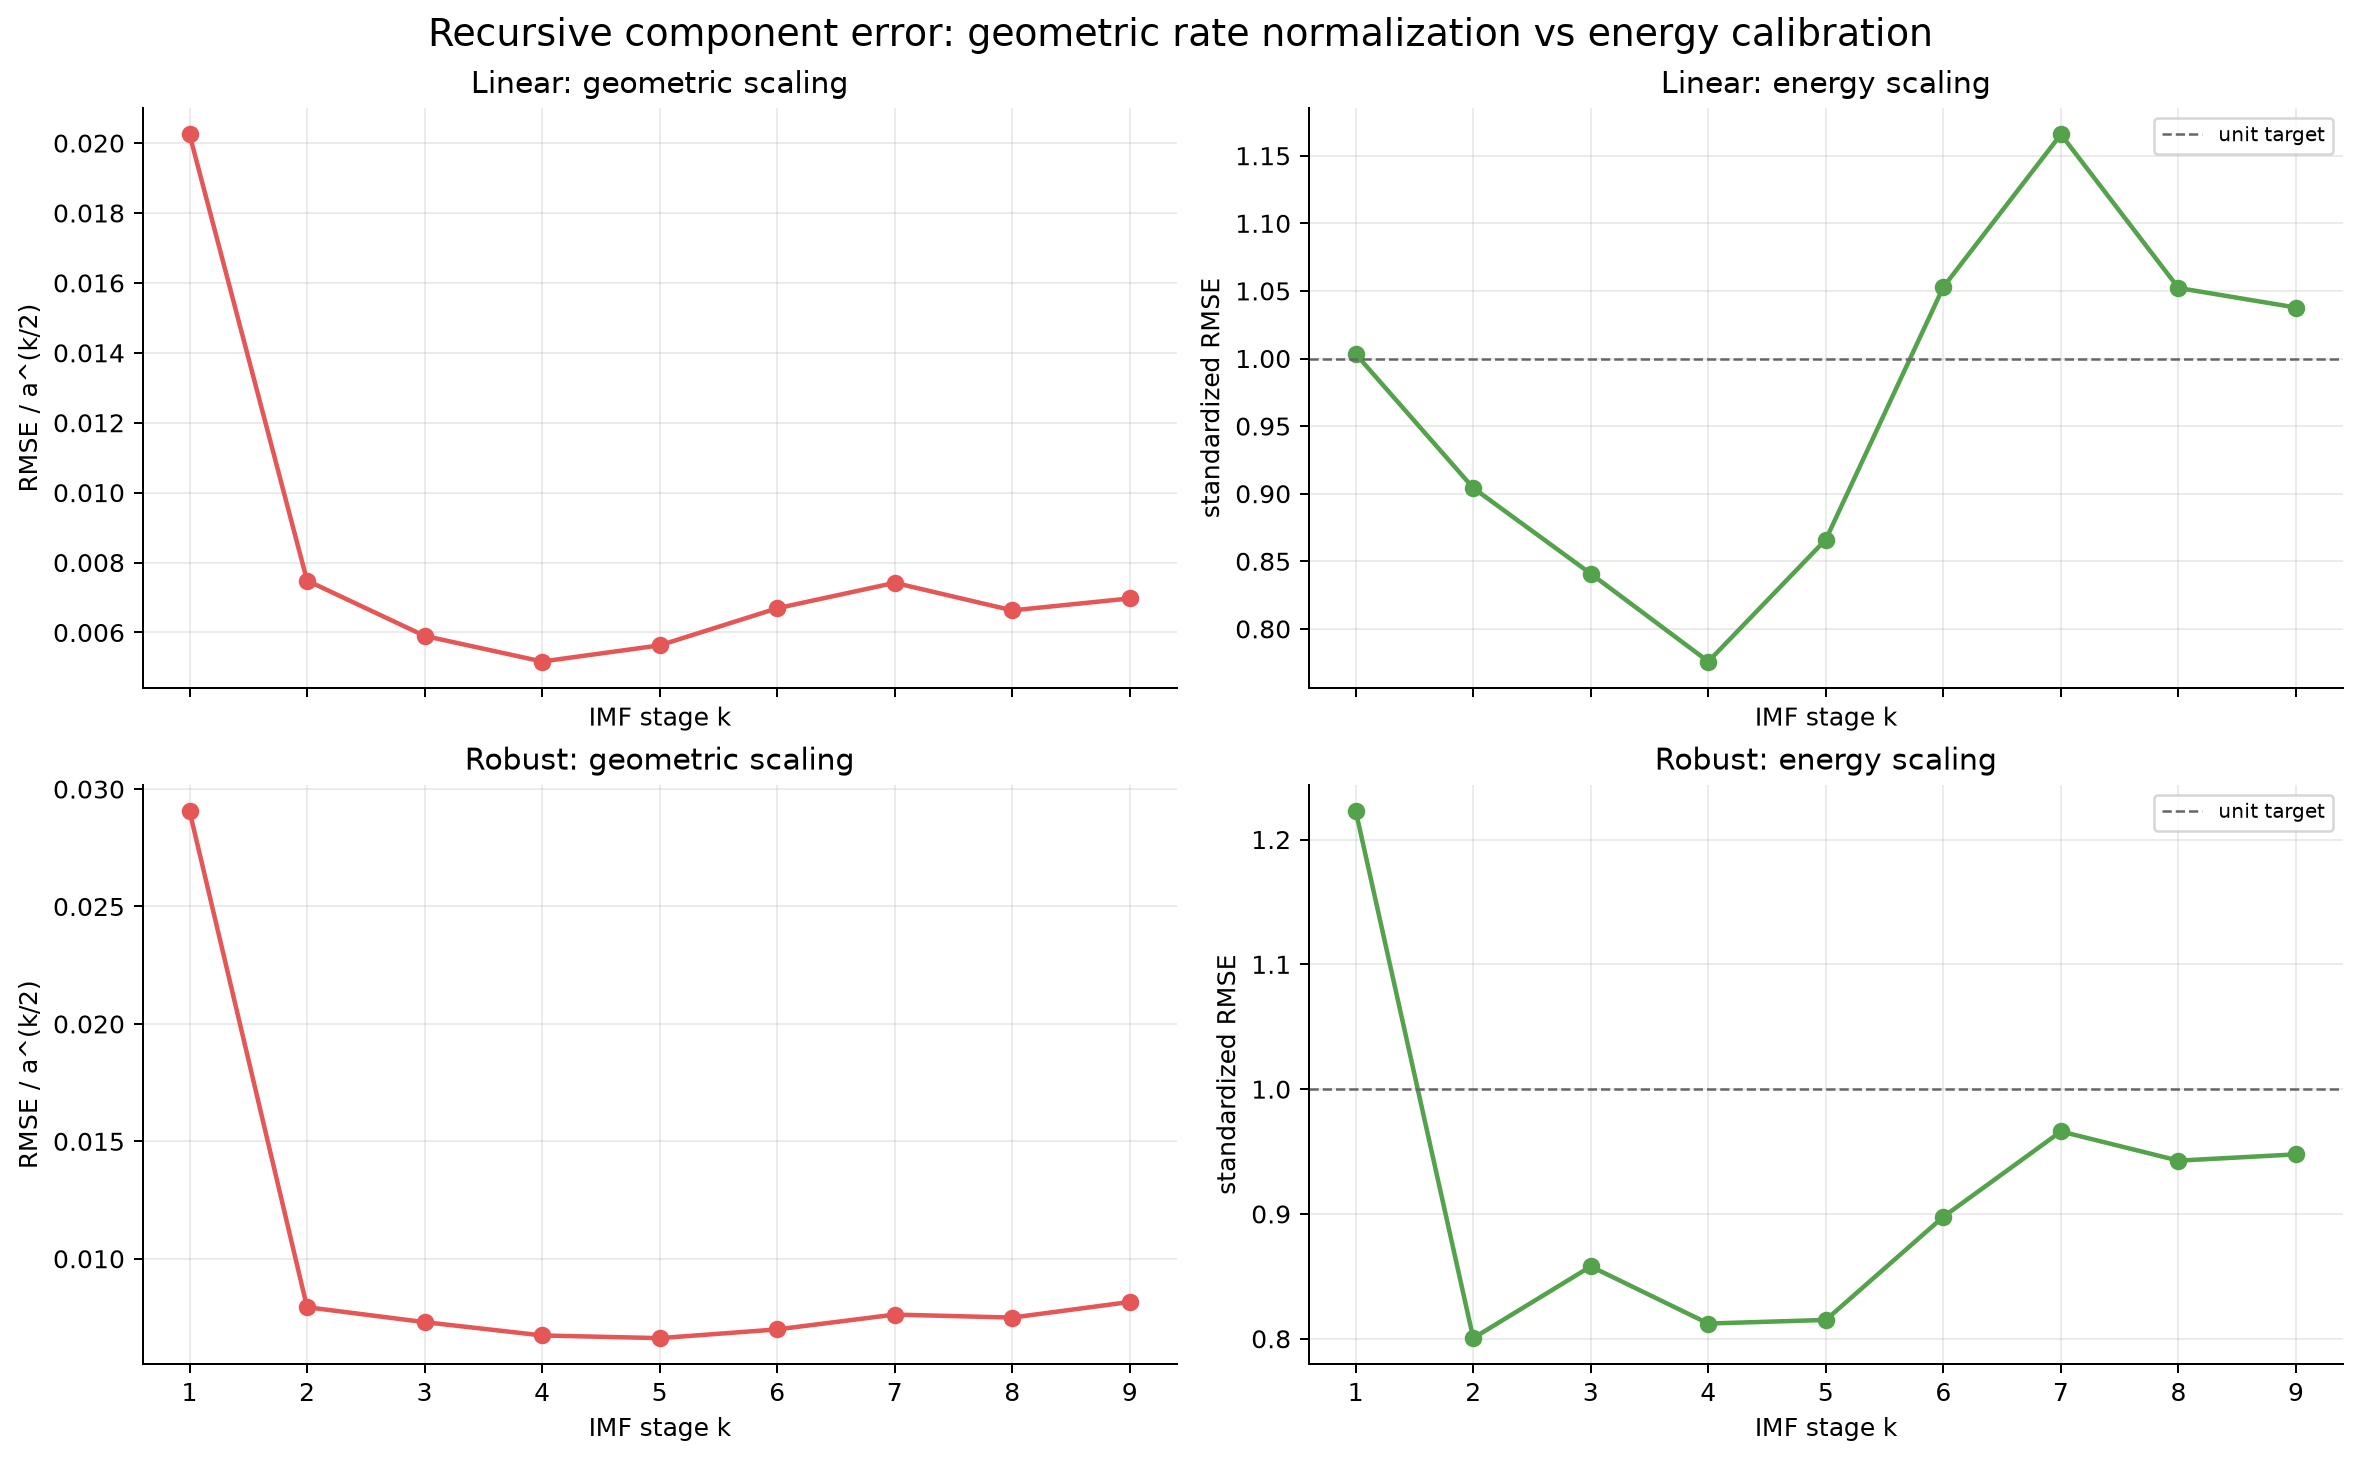
\includegraphics[width=\linewidth]{figures/gd_imf_error_scaling_comparison/recursive_rmse_scaling_comparison.png}
\caption{Recursive component-error RMSE under geometric bandwidth scaling and
stage-specific energy scaling. The dashed line in each energy panel is the unit
calibration target. The geometric panels retain the stage-dependent filter-energy
constant, while the energy panels divide by it.}
\label{fig:recursive-scaling-comparison}
\end{figure}

\begin{table}[H]
\centering
\small
\begin{tabular}{@{}>{\raggedright\arraybackslash}p{0.10\linewidth}rrrr@{}}
\hline
Stage & Linear geometric & Linear energy & Robust geometric & Robust energy \\
\hline
1 & 0.020249 & 1.003 & 0.029067 & 1.223 \\
2 & 0.007485 & 0.904 & 0.007936 & 0.800 \\
3 & 0.005903 & 0.841 & 0.007300 & 0.858 \\
4 & 0.005170 & 0.776 & 0.006733 & 0.812 \\
5 & 0.005631 & 0.866 & 0.006619 & 0.815 \\
6 & 0.006692 & 1.053 & 0.006990 & 0.898 \\
7 & 0.007421 & 1.166 & 0.007622 & 0.966 \\
8 & 0.006632 & 1.052 & 0.007494 & 0.943 \\
9 & 0.006974 & 1.038 & 0.008159 & 0.948 \\
\hline
\end{tabular}
\caption{Recursive RMSE after geometric or energy scaling.}
\label{tab:stage-values}
\end{table}

The stage-one-to-tail ratio is defined by
\[
R_{1:\mathrm{tail}}
=\frac{r_1}{\frac{1}{8}\sum_{k=2}^{9}r_k},
\]
where $r_k$ is the scaled recursive RMSE. Flatness is summarized by the sample
coefficient of variation
\[
\CV(r_1,\ldots,r_9)=\frac{\operatorname{sd}(r_1,\ldots,r_9)}
{\operatorname{mean}(r_1,\ldots,r_9)}.
\]
In this document, ``flat'' has a narrow meaning: the scaled recursive RMSE is
approximately unchanged as the stage index $k$ changes. It does not mean that
the raw errors are small or that the recovered components are accurate. A
perfectly flat nine-stage sequence would have $R_{1:\mathrm{tail}}=1$ and
$\CV=0$. Thus $|R_{1:\mathrm{tail}}-1|$ measures the special mismatch of stage
1 relative to stages 2--9, while the CV measures variation over all nine
stages. Values closer to zero in Figure~\ref{fig:recursive-flatness-comparison}
mean that one scaling rule gives the stages a more uniform error scale.

\begin{table}[H]
\centering
\small
\begin{tabular}{@{}>{\raggedright\arraybackslash}p{0.16\linewidth}
>{\raggedright\arraybackslash}p{0.22\linewidth}rrr@{}}
\hline
Method & Case & $R_{1:\mathrm{tail}}$ & CV, stages 1--9 & CV, stages 2--9 \\
\hline
Geometric & Linear recursive & 3.121 & 58.0\% & 13.0\% \\
Energy & Linear recursive & 1.043 & 13.0\% & 13.9\% \\
Geometric & Robust recursive & 3.951 & 74.3\% & 7.5\% \\
Energy & Robust recursive & 1.390 & 14.2\% & 7.7\% \\
\hline
\end{tabular}
\caption{Numerical ingredients of the flatness comparison. The ideal values are
$R_{1:\mathrm{tail}}=1$ and CV $=0$.}
\label{tab:flatness}
\end{table}

\begin{figure}[H]
\centering
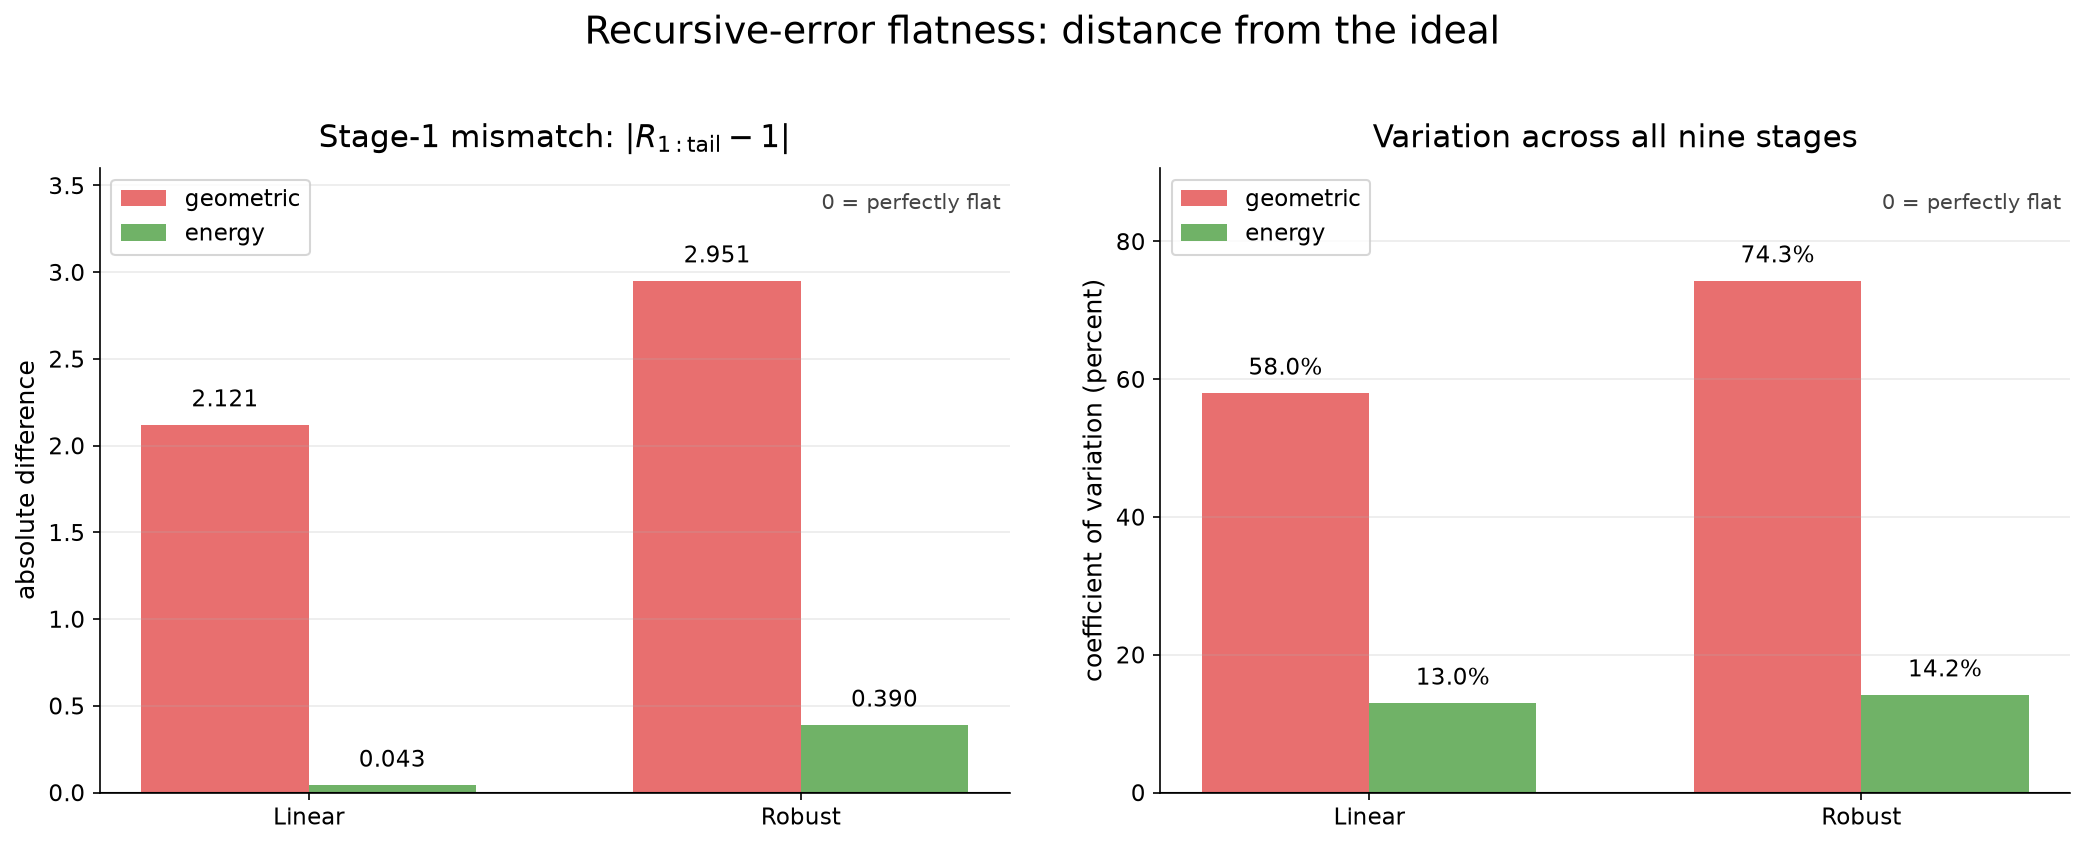
\includegraphics[width=0.95\linewidth]{figures/gd_imf_error_scaling_comparison/recursive_flatness_comparison.png}
\caption{Recursive error flatness. The left panel plots
$|R_{1:\mathrm{tail}}-1|$, so zero means that stage 1 has the same scaled RMSE
as the mean of stages 2--9. The right panel plots the coefficient of variation
over all nine scaled RMSE values, where zero means that every stage has exactly
the same value. Smaller bars indicate a more uniform stage-to-stage scale, not
smaller raw errors.}
\label{fig:recursive-flatness-comparison}
\end{figure}

For the linear recursive series, energy scaling changes the stage-one-to-tail
ratio from $3.121$ to $1.043$. For the robust series, it changes the ratio from
$3.951$ to $1.390$. The remaining robust difference is plausible for one fixed
noise realization and a scale estimated from only 32 bootstrap replicates; it
should be assessed across repeated observations rather than forced to equal one.

The tail CV is not materially reduced because stages 2--9 were already close to
a common lower plateau under geometric scaling. The main benefit of energy
scaling is therefore not generic smoothing of the curve: it corrects the
structural mismatch between the first low-pass component and the later
band-pass components.

\section{Recommended Comparison Protocol}

A fair evaluation should use the same raw component errors and apply both
normalizations afterward.

\begin{enumerate}
    \item Show both the geometric rate-normalized recursive error and the
    energy-standardized error; do not silently replace one interpretation with
    the other.
    \item Report results for all stages and for the tail stages $k\geq2$ or
    $k\geq3$. This separates initialization effects from steady multiscale
    behavior.
    \item For each method, report:
    \begin{itemize}
        \item stage-one-to-tail ratio;
        \item all-stage and tail-stage coefficient of variation;
        \item mean and range of standardized RMSE;
        \item computational time and, for robust scaling, bootstrap uncertainty.
    \end{itemize}
    \item Repeat the experiment across noise seeds. For energy scaling, check
    whether $\E[\RMSE(z_k)^2]$ is close to one, not whether every realized
    $\RMSE(z_k)$ equals one.
    \item Compare linear and robust methods on matched Gaussian-only and
    contaminated observations if the goal is method comparison.
    \item Evaluate sup errors separately. A suitable comparison can use
    stage-specific bootstrap quantiles of $\lVert e_k\rVert_\infty$ or a
    simultaneous confidence-band normalization.
\end{enumerate}

\section{Recommendation}

Both methods should be retained because they diagnose different properties.

\begin{itemize}
    \item Use geometric scaling as a compact theoretical-rate diagnostic and to
    compare with statements of order $(nh_k)^{-1/2}$.
    \item Use energy scaling as the primary stage-to-stage calibration for
    recursive IMF errors. It correctly accounts for the low-pass first
    component and the lower-energy band-pass components that follow.
    \item For the robust decomposition, increase the bootstrap size and report
    Monte Carlo uncertainty before using the energy scales for formal inference.
    \item Do not interpret either RMS normalization as a proof of constant sup
    error.
\end{itemize}

The clearest presentation is a side-by-side pair of plots: geometric scaling on
the left, labeled ``bandwidth-order normalization,'' and energy scaling on the
right, labeled ``stage-specific RMS calibration.''

\section{Reproducibility Files}

\begin{itemize}
    \item Original geometric-scaling notebook:
    \path{gd_imf_real_vs_calculated.ipynb}.
    \item Energy-scaled reproduction:
    \path{output/jupyter-notebook/}\\
    \path{gd_imf_real_vs_calculated_energy_scaled.ipynb}.
    \item Investigation summary:
    \path{research/first-imf-recursive-error/executive-summary.md}.
    \item Detailed theory review:
    \path{research/first-imf-recursive-error/agents/theory.md}.
\end{itemize}

\begin{thebibliography}{9}

\bibitem{nadaraya1964}
E.~A. Nadaraya.
On estimating regression.
\emph{Theory of Probability and Its Applications}, 9(1):141--142, 1964.
\href{https://doi.org/10.1137/1109020}{doi:10.1137/1109020}.

\bibitem{watson1964}
G.~S. Watson.
Smooth regression analysis.
\emph{Sankhy\={a}: The Indian Journal of Statistics, Series A},
26(4):359--372, 1964.
\href{https://www.jstor.org/stable/25049340}{JSTOR 25049340}.

\bibitem{fan-gijbels1996}
J. Fan and I. Gijbels.
\emph{Local Polynomial Modelling and Its Applications}.
Chapman \& Hall, London, 1996.

\bibitem{tsybakov2009}
A.~B. Tsybakov.
\emph{Introduction to Nonparametric Estimation}.
Springer, New York, 2009.
\href{https://doi.org/10.1007/b13794}{doi:10.1007/b13794}.

\bibitem{spokoiny2026}
V. Spokoiny.
\emph{Intrinsic robust multiscale filtering}.
Unpublished project draft, July 3, 2026, especially Lemma~2.5.

\end{thebibliography}

\end{document}
